\documentclass[border=0.5mm]{standalone}

\usepackage{import}
\subimport{../../../}{preamble.tex}

\usepackage{tikz}
\usetikzlibrary{calc}

\usepackage{pgfplots}
\usepgfplotslibrary{fillbetween}

\begin{document}

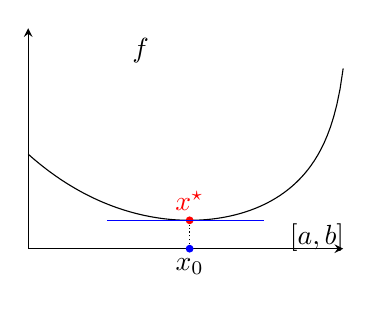
\begin{tikzpicture}

  \begin{axis}[
    ticks=none,
    axis lines=left,
    y=0.8cm,            % y unit vector
    x=2cm,            % x unit vector
    clip=false,
    ymax=4,
    ymin=0.5,
    xlabel={$[a, b]$},
    ylabel={$f$},
    x label style={at={(axis description cs:0.8,0.05)},anchor=west},
    y label style={at={(axis description cs:0.3,0.8)},rotate=-90,anchor=south west},
    ]
    
    \addplot[mark=none, black, samples=100, domain=-1:1] {exp(-1*x) - ln(1.05-x) };

    \node[circle, inner sep=1, fill=red] (xstar) at (axis cs:0.024844,0.95062) {};
    \node[above, red] at (xstar) {$x^\star$};


    \addplot[mark=none, blue, samples=100, domain=-0.5:0.5] {0.95062+(x-0.024844)*0};
    \node[circle, inner sep=1] (f0) at (axis cs:0.024844,0.95062) {};
    \node[circle, inner sep=1, fill=blue] (x0) at (axis cs:0.024844,0.5) {};
    \node[below] at (x0) {$x_0$};
    \draw[densely dotted] (x0) -- (f0);
    
  
    % \node[above] at (xstar) {$x_0$};
    
  \end{axis}
  
\end{tikzpicture}

\end{document}

%%% Local Variables:
%%% mode: latex
%%% TeX-master: t
%%% End:
